\documentclass[11pt]{article}
\usepackage{amssymb,amsfonts,epsfig,algorithm,algorithmic,url}
\usepackage{caption,subcaption,amsmath}
\usepackage{cite}
\usepackage{titling}
\textheight 8.8truein
\parskip 0.1in
\topmargin -0.5truein
\textwidth 6.5truein
\oddsidemargin -0.05in
\evensidemargin -0.05in
% \renewcommand{\baselinestretch}{1.2}   %line space adjusted here
\setcounter{footnote}{0}
\sloppy

\usepackage[nottoc]{tocbibind}

\renewcommand{\theequation}{\thesection.\arabic{equation}}
\newcommand{\newsection}{\setcounter{equation}{0}\section}

\newtheorem{theorem}{Theorem}
\newtheorem{proposition}[theorem]{Proposition}
\newtheorem{lemma}[theorem]{Lemma}
\newtheorem{corollary}[theorem]{Corollary}
\newtheorem{definition}[theorem]{Definition}
\newtheorem{example}[theorem]{Example}

\begin{document}
\title{\bf CSCI 8551 Intelligent Agents Course Project\\
Final report\\
Refined Model in Python: the Thriving of Punishers
}
\date{\today}
\author{Bolei Di, Xi Guo}
\maketitle

\section{Indtroduction}
%read the following section to see if it makes sense
Punishment in a society allowing voluntary cooperation has been evolving for more than two thousand years \cite{morris1995oxford}. Public punishment by paying a personal cost has proved to be an important mechanism that facilitates the cooperation of humans \cite{hauert2007via}. In the study of Hauert \textit{et al}., a model has been exploited to show the evolutionary merits of punishment. Emergence of punishers can be achieved when joining the cooperation is voluntary. The study of Hauert et al. was based on several assumptions that may not represent the characteristics of human organizations. Specifically, the original model were created in an ideal environment in which each agent has the full access to the performance of other agents. The agents were also not obligated in contributing to the punishment. However, we thought of two examples that contradicts these assumptions in the model. 1) The restricted communication infrastructure in ancient time (such as beacon) provided incomplete information, which people made their decisions based upon. 2) One of the functions of the obligated tax system is to establish the institutes for enforced punishment, including police and jails. To address these limitations in the original model, in this study, we attempted to rebuild the model and enhance the model in order to explore the theoretical aspects of the situations described above.

We planned to add the following variations in the new model. 1) Geographical constraints of the agents. 2) Enforced insurance (or tax) policy for each agents in the society. 3) Combining the geographical constraints and the insurance policy. We proposed to achieve three goals: 1) To replicate the original result; 2) To build enhanced model by incorporating information constraints and the enforced insurance policy; 3) To examine the impact of variations and parameters on the current model.

\section{Game Model}
The game model consists of three parts which forms a loop that enables running the model for infinete steps as in Figure \ref{fig:game_model}. Game type determines the reward to each type of agents given a population of agents. Information structure determines the feedback each agent sees based on rewards. Transition probability takes in the feedback of each agent and output its probabilities of transforming into different types of agents. Given each different method for each step, this model can simulate any combination of the three steps.

\begin{figure}[!h]
  \centering
  \caption{Overview of game model}
  \label{fig:game_model}
  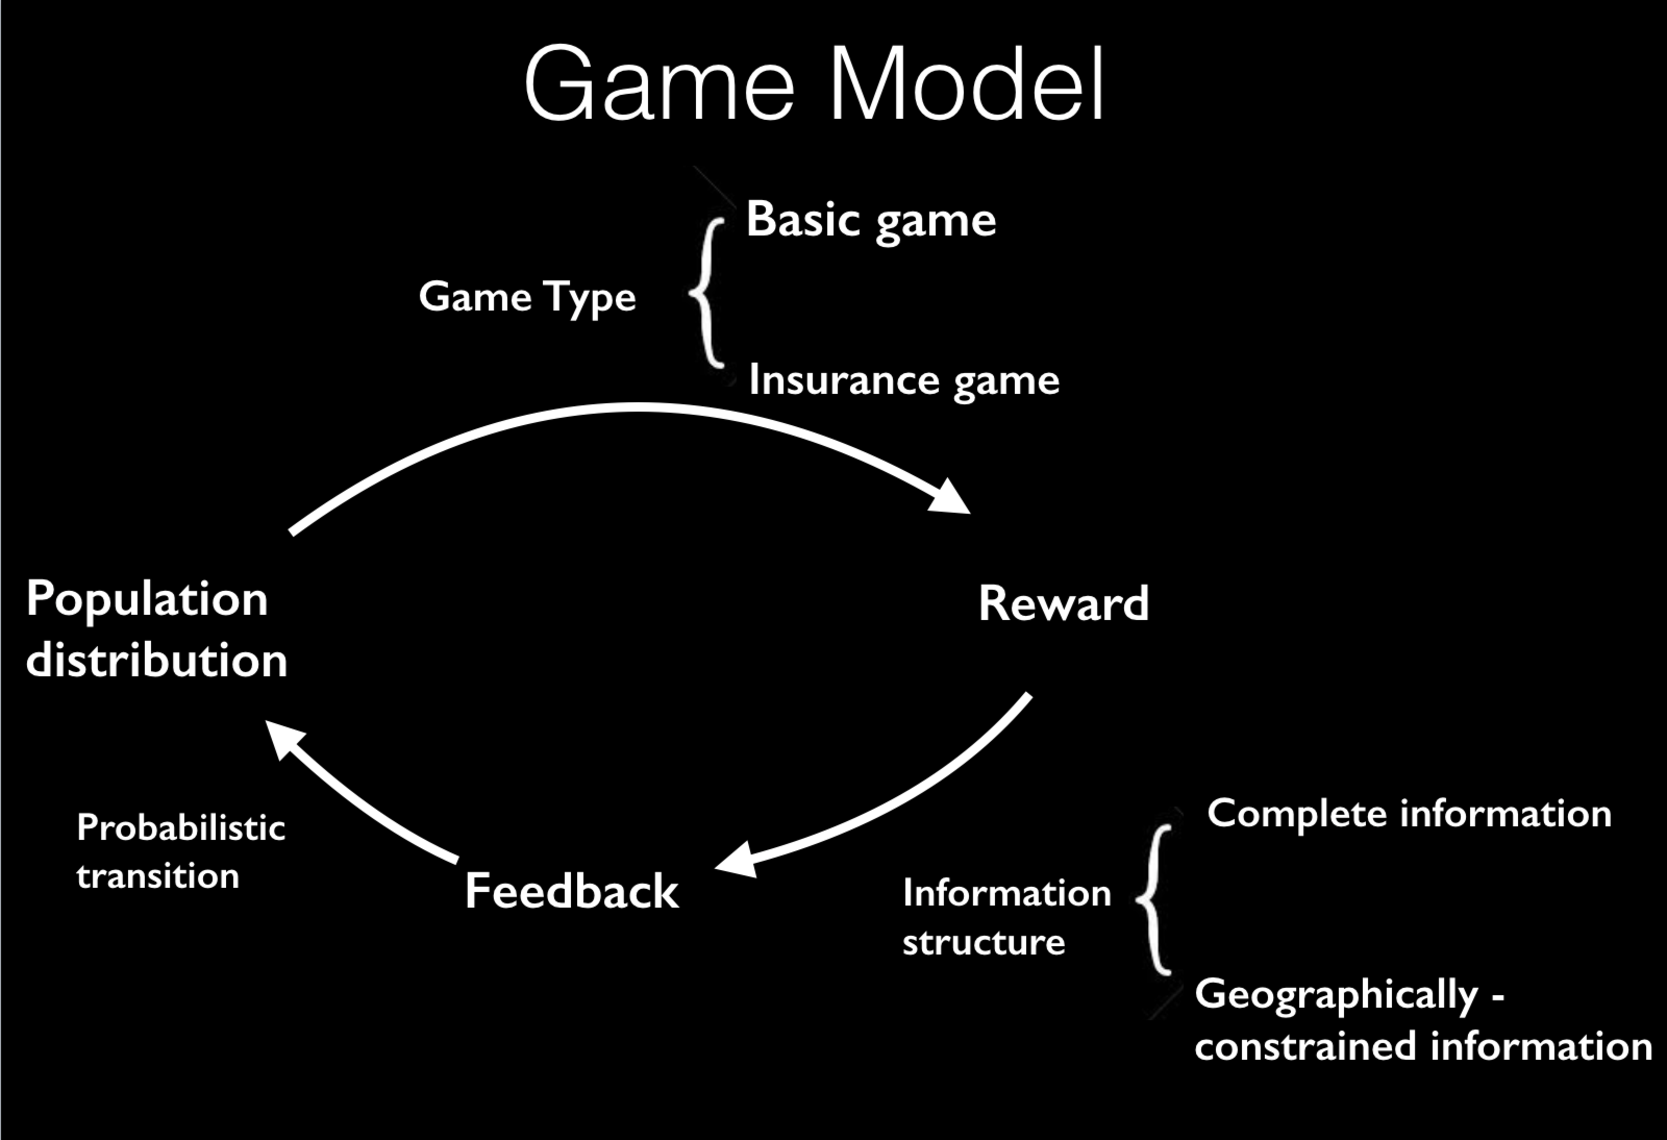
\includegraphics[scale=0.4]{game_model.pdf}
\end{figure}

\subsection{Game type}\label{sec:game_type}
Here we consider two game types for the experiments - basic game and enforced insurance game. We use $R_n,R_c,R_p,R_d,n,c,p,d$ to denote the rewards and populations for non-participant, cooperator, punisher and defector. $l$ denotes the contribution of cooperators and punishers' contribution to the cooperation. $\gamma$ denotes the cost of punishment for each punisher and $\beta$ denotes the punishement a defoctor receive from each punishement. $t$ is the tax or insurance paid by each member in the cooperation in insurance game. Rewards of a basic and insurance game is defined as:
\begin{align}
s &= c + p + d \\
R_n &= \sigma \\
R_c &= r(c+p)l/s - l - \{t\} \\
R_p &= r(c+p)l/s - l - d\gamma - \{t\}\\
R_d &= r(c+p)l/s - p\beta + \{ t(c+p)/d \}
\end{align}
where the terms in $\{\}$ are included only in insurance game. All the results shown later in this report share the same set of parameter values: $\sigma=1,r=5,l=1,\beta=2,\gamma=0.1,t=0.1$. These parameters are carefully tuned, such that, 1) having one punisher in the cooperation, cooperators' rewards would be higher than defectors, 2)non-participants receive much lower (one fourth) rewards than anyone in a healthy (few defectors) cooperation, 3) a punishment is very cost-effective and 4) a tax/insurance paid by members is only a small fraction of rewards in healthy cooperation.

\subsection{Information structure}
For the basic game, the above information is seen by all agents, and for the geographically constrained game, an agent only sees its neighbors' rewards and only knows about types of agents of itself and its neighbors. For our geographically constrained simulations, the game is played in a 50 by 50 rectangle region and the visibility radius is 10.

\subsection{Probabilistic transition}
The transition function determines the probabilities of transforming into other agent types given the feedback an agent sees. We have several transition function but only one worked out well. The transition function distinguishes between two states of agents, ignorance and non-ignorance. An ignorance agent sees only type and rewards of its own kind, has 99.7\% chance staying as is and 0.3\% chance transforming into other agents. For a non-ignorance agent, it still has 80\% chance of staying as is, 1\% for each type it does not see, and the rest close to 20\% is splitted proportionally to the sigmoid function of the differences between its own reward and other agent types' reward it can see.

\section{Experimental Results}
In the following sections, we will illustrate the results from the basic game, enforced insurance game and geographically constrained game. We will discuss the effect of these two features.
\subsection{Basic game}
%%%add a sentence in the parenthesis, describe other parameters, as I don't know the notation of them.
As shown in Figure 1(a) and Figure 1(b), the basic game is initialized with 100 defectors. (Other parameters need to be listed here) We observed the similar trend of the successful evolution of punishers after 100 transitions. Both cooperators and punishers have survived in the end and maintained in a stable state. Unlike Figure 1A in the original paper, we failed to observe the dominant trend of a overly large number of punishers even after 1000 transitions (Figure 1(c)). The possible explanation for the distinction of the number of punishers is that the transition function that we used allows a smaller number of emerging defectors, thus the system does not require a large number of punishers to reach to the steady state. Furthermore, we have observed the similar oscillation transient of non-participants, cooperators and defectors. This transient period is from the starting point to the point when the system reaches to a stable state.

 %%%%%%%%%%%%%
\begin{figure}[!h]
  \caption{Basic game}
  \begin{subfigure}{.5\textwidth}
    \centering
    \caption{The evolution of agents: basic game}
    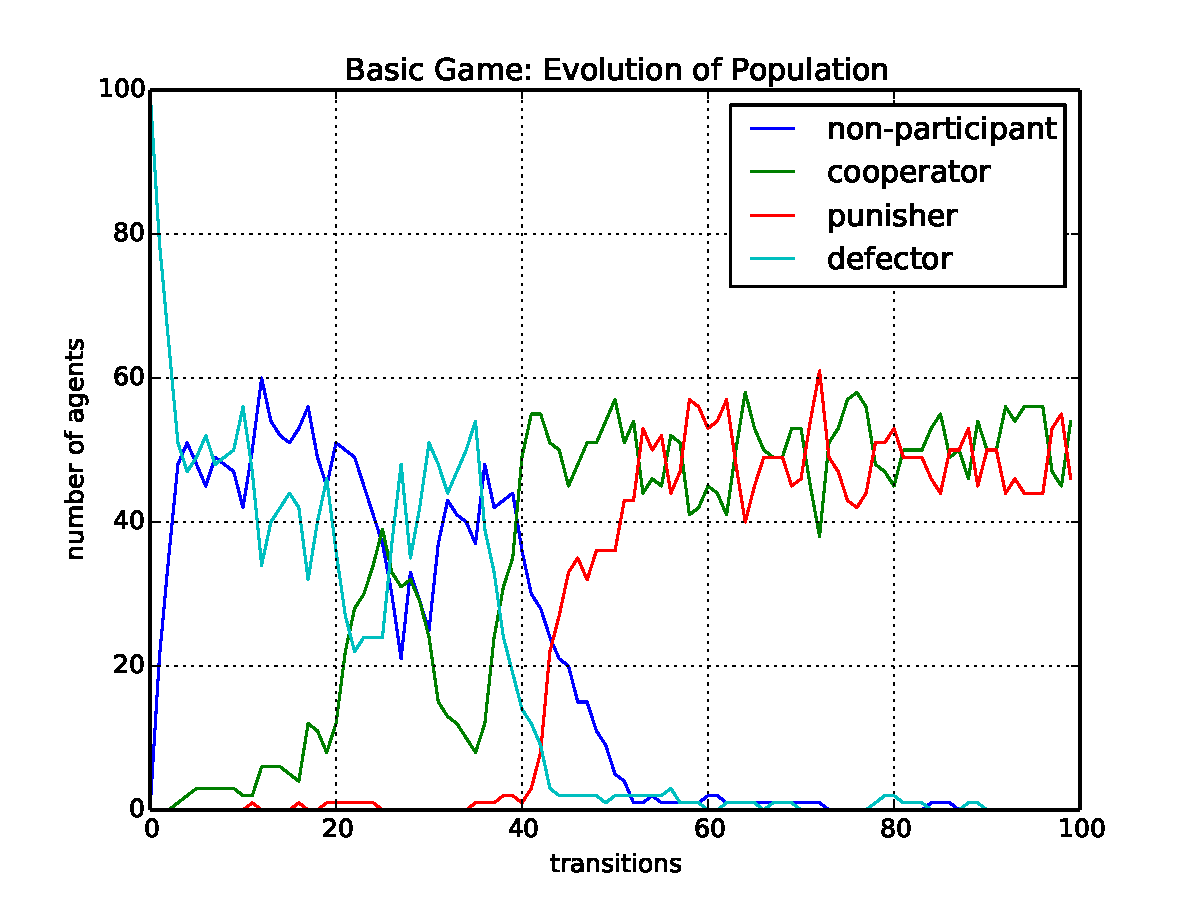
\includegraphics[scale = 0.4]{1.pdf}
  \end{subfigure}
  \begin{subfigure}{.5\textwidth}
    \centering
    \caption{The Evolution of rewards: basic game}
    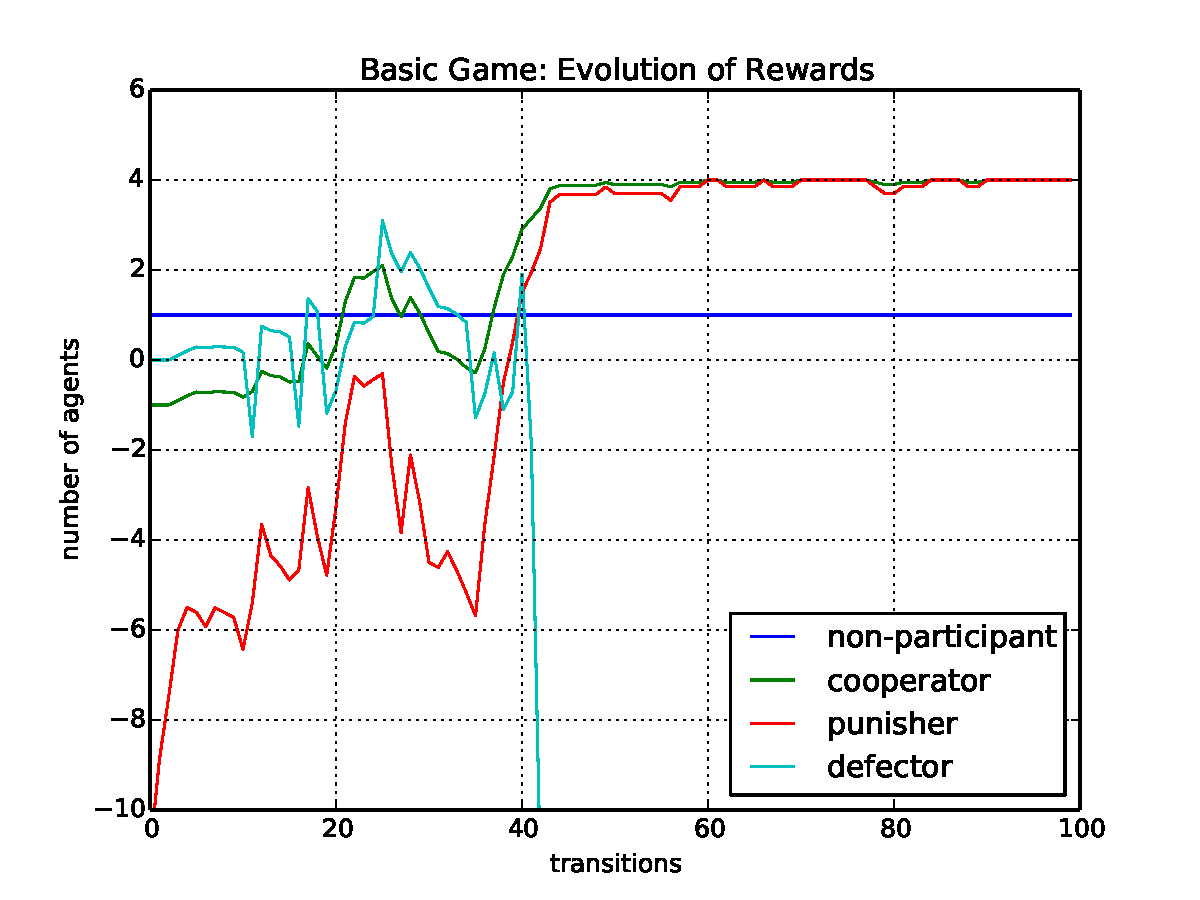
\includegraphics[scale = 0.4]{2.pdf}
  \end{subfigure}
  \begin{subfigure}{1\textwidth}
    \centering
    \caption{Results of basic game (1000 transitions)}
    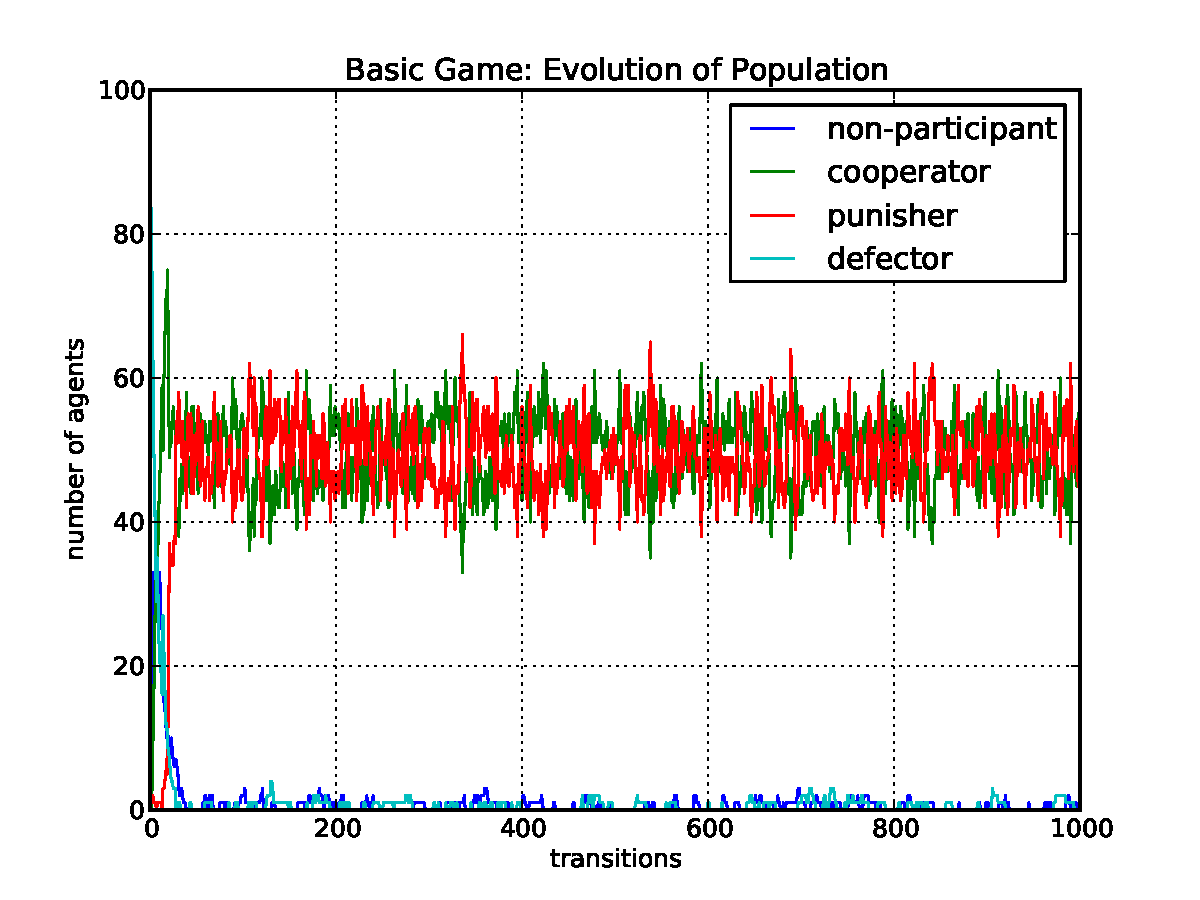
\includegraphics[scale = 0.4]{3.pdf}
  \end{subfigure}
\end{figure}
 %%%%%%%

\subsection{Effect of geographic constraints}
%%%%%read this paragraph to see if it makes sense
Geographic constraint worked as a inhibitor in the process of evolution. It increased the oscillation of the number of agents and sometimes it could slow down the propagation of one or more types of rewarding agents. Comparing Figure 1(a) and Figure 2(a), we discovered that same initialization condition has led to almost the same lengths of the transient period (about 60 transitions). The population distribution exhibited higher fluctuation in the geographically constrained game. The constrain could further slow down the propagation of one or more types of rewarding agents, as its good performance was not seen by its neighbor agents. Figure 3(a) and Figure 3(b) are two snapshots of the distribution of agents in the game corresponding with Figure 2. The gray circle indicates an agent has been transformed to punisher at 17th iteration. Although the reward of punishers at this point was as high as that of defectors', being restricted by the geographic constraint, the punisher was not able to influence its neighboring agents. It changed to a defector in the subsequent transition.
%%%%%%%%%%
\begin{figure}[!h]
 \caption{Basic geographically constrained game}
 \begin{subfigure}{.5\textwidth}
   \centering
   \caption{The evolution of agents: basic geographically constrained game}
   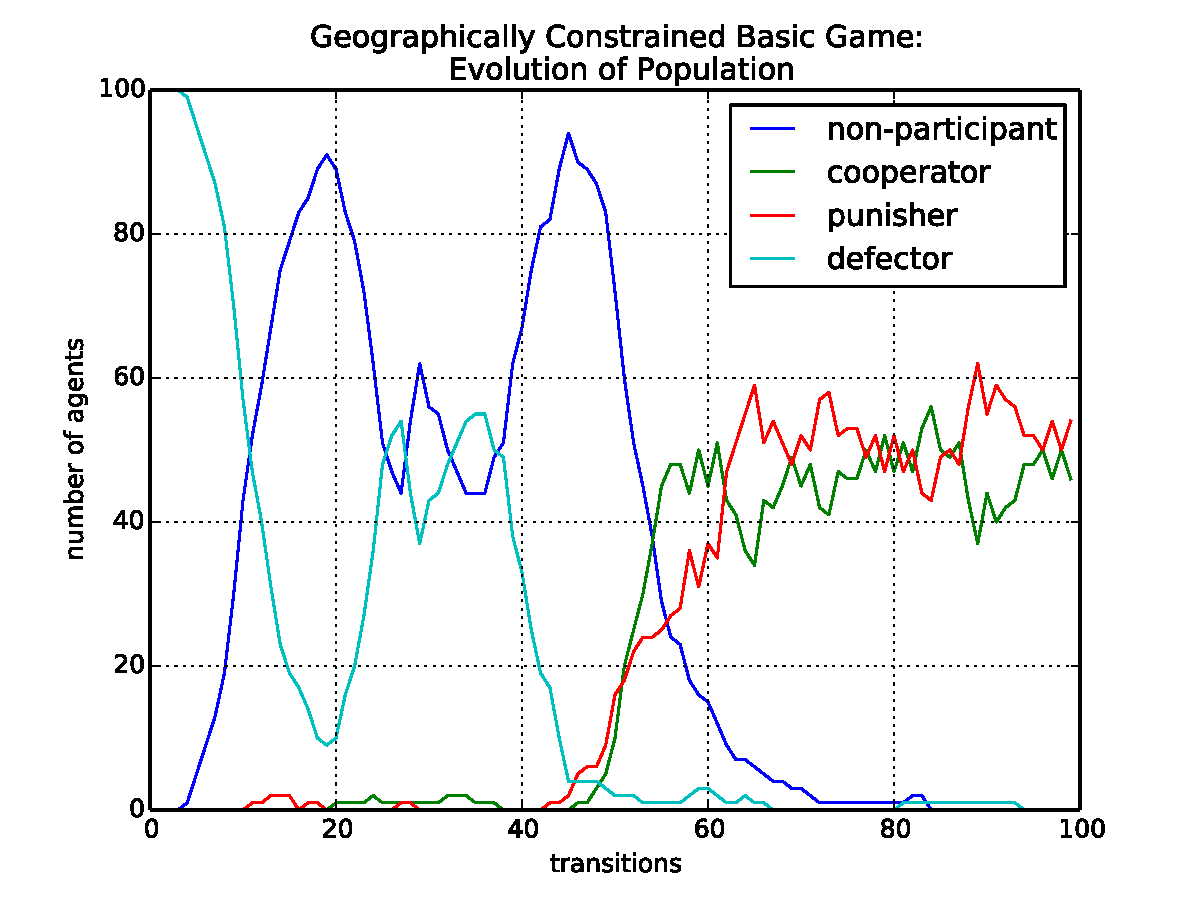
\includegraphics[scale = 0.4]{4.pdf}
 \end{subfigure}
 \begin{subfigure}{.5\textwidth}
   \centering
   \label{}
   \caption{The evolution of rewards: basic geographically constrained game}
   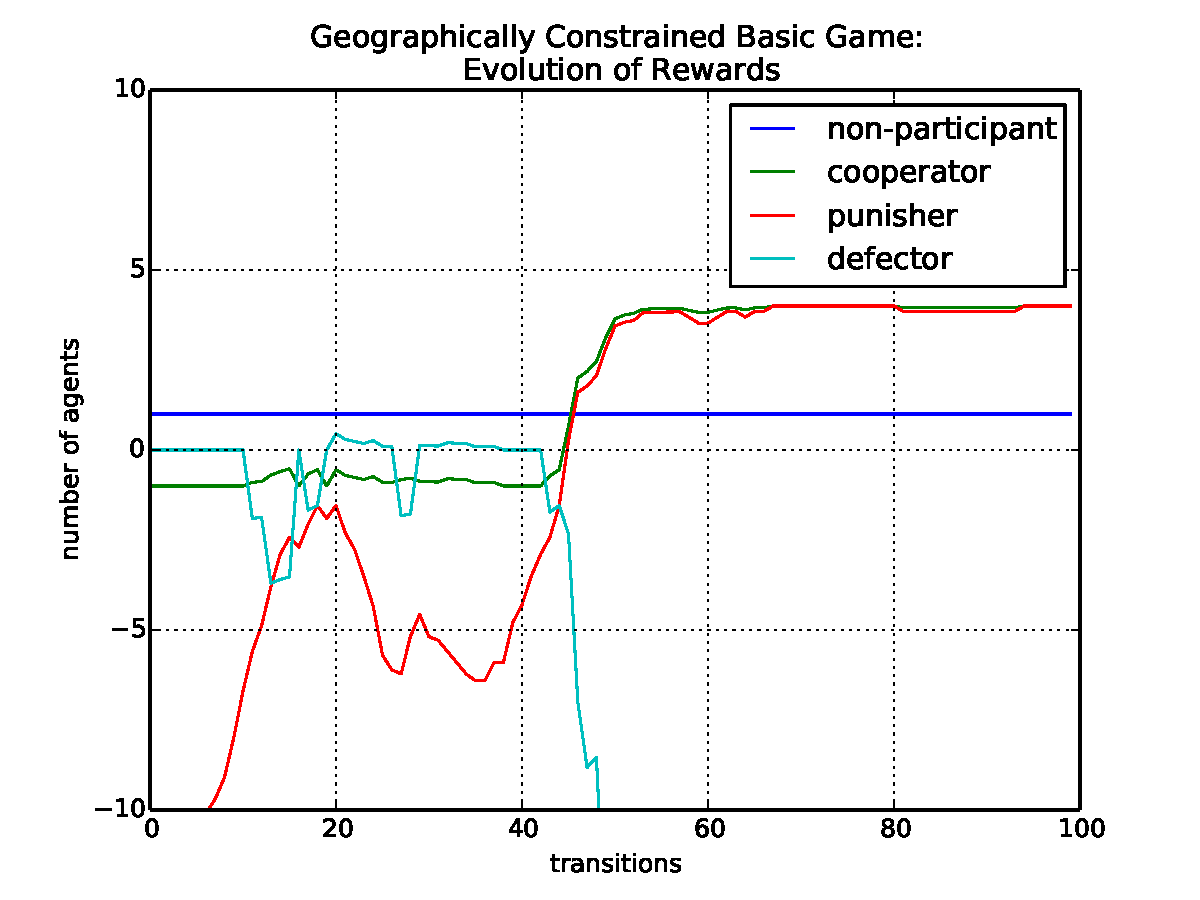
\includegraphics[scale = 0.4]{5.pdf}
 \end{subfigure}
\end{figure}
%%%%%%%%%%
%%%%%%%%%%
\begin{figure}[!h]
 \caption{The distribution of agents in geographically constrained game}
 \begin{subfigure}{.5\textwidth}
   \caption{The distribution at 17th transition}
   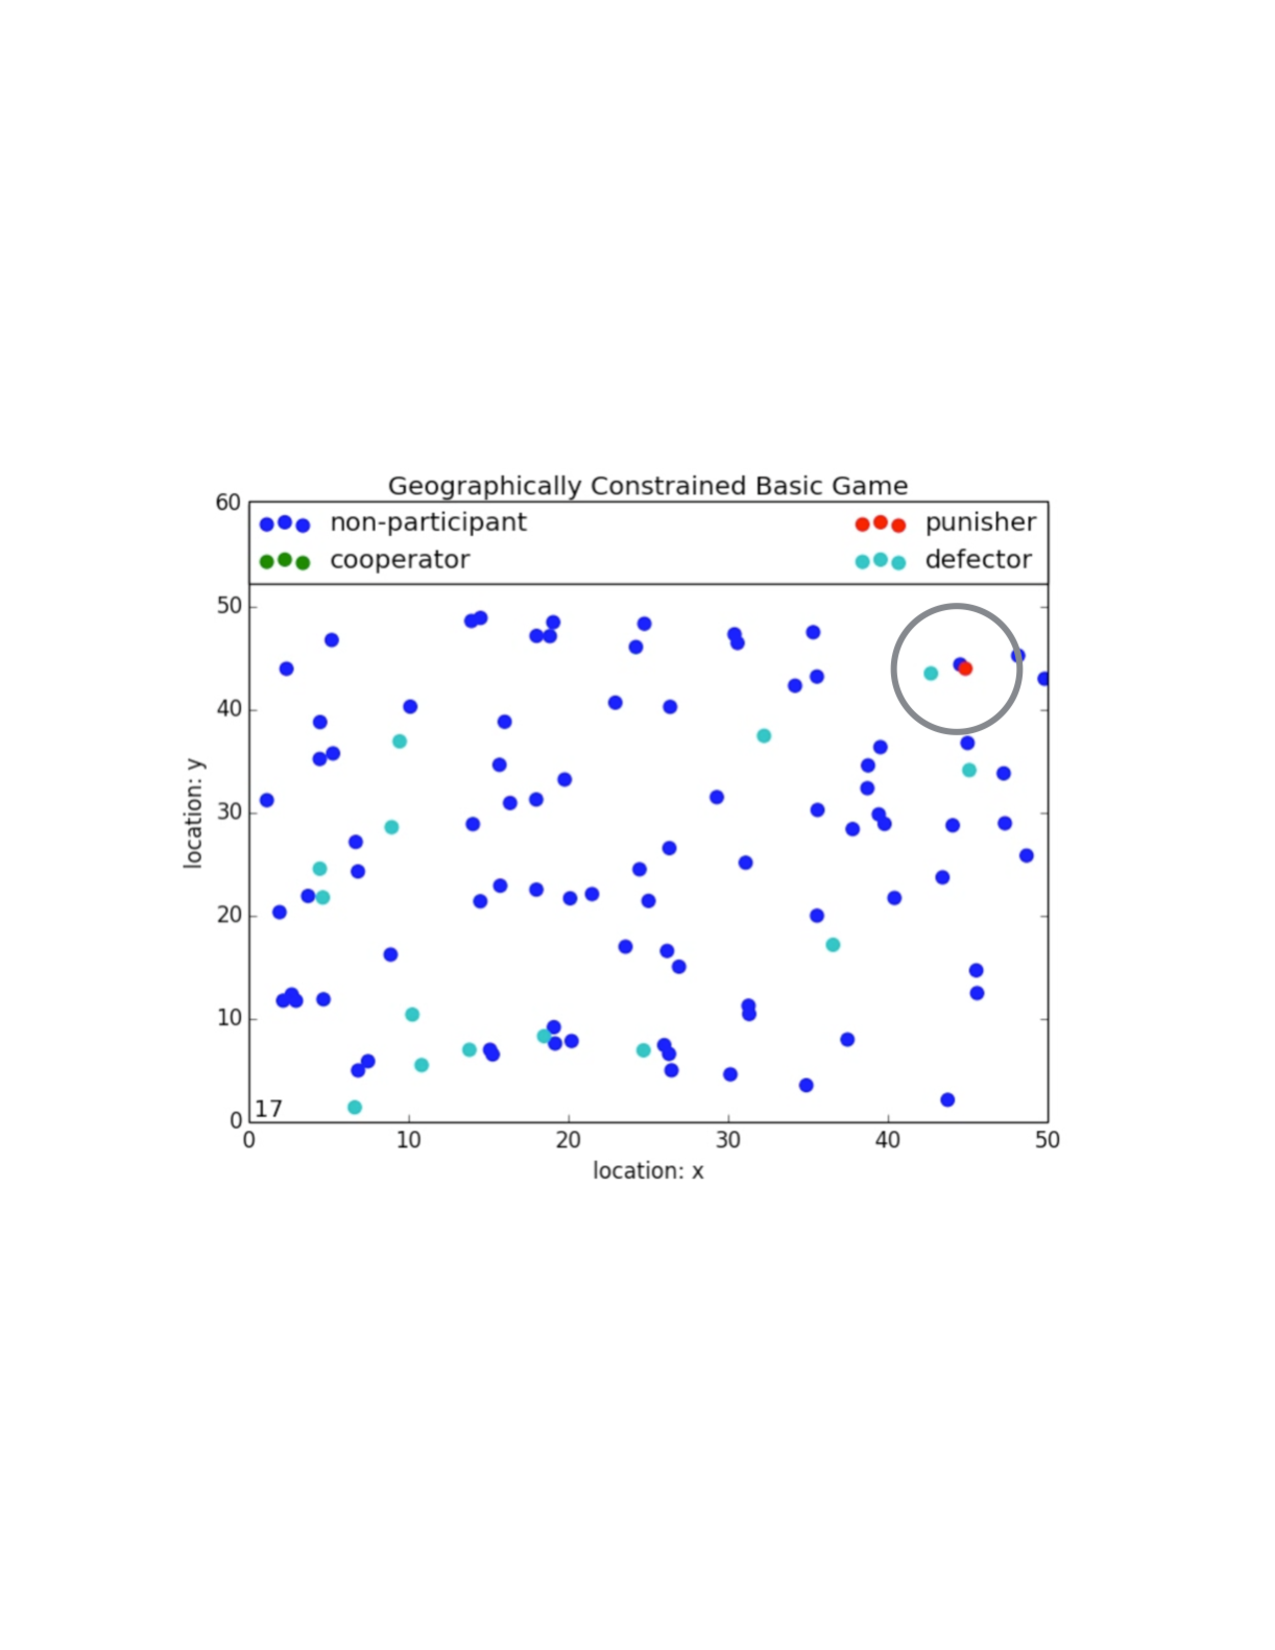
\includegraphics[scale = 0.4]{8.pdf}
 \end{subfigure}
 \begin{subfigure}{.5\textwidth}
   \label{}
   \centering
   \caption{The distribution at 18th transition}
   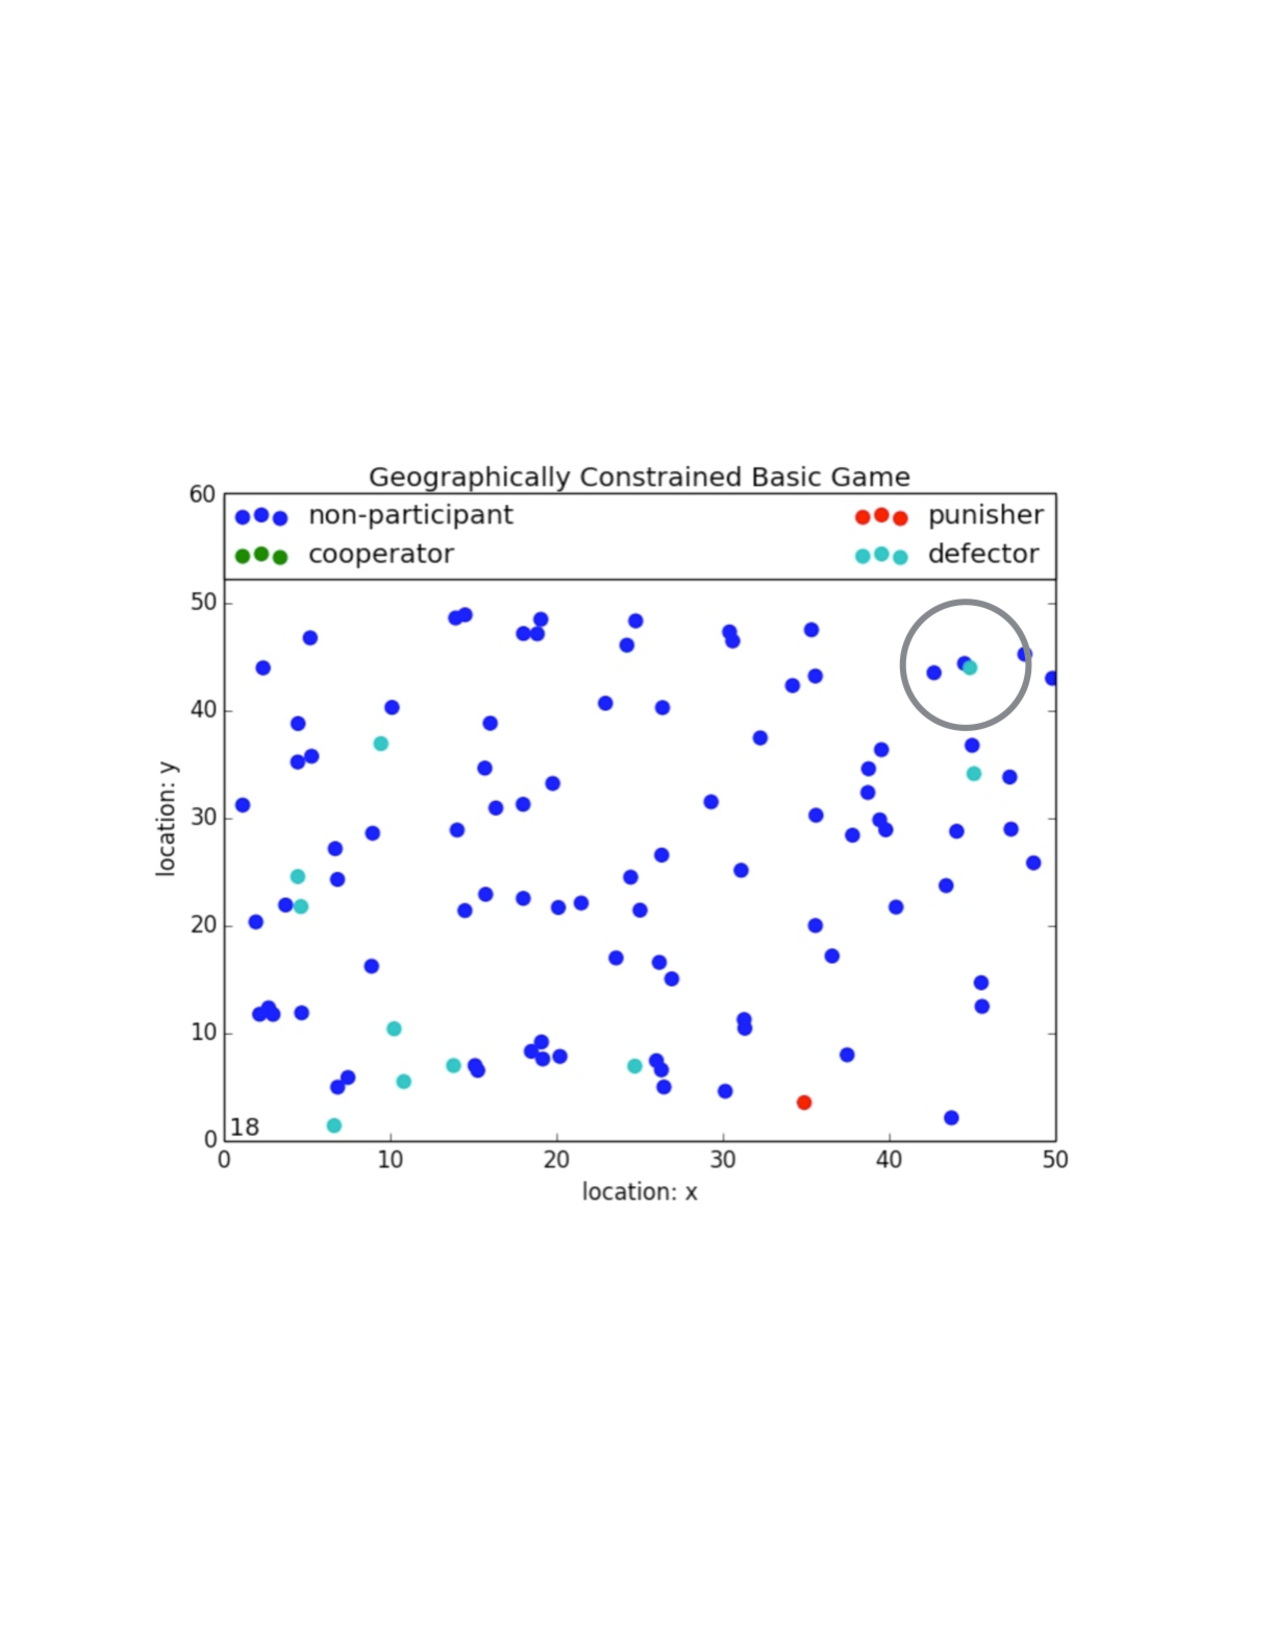
\includegraphics[scale = 0.4]{9.pdf}
 \end{subfigure}
\end{figure}
%%%%%%%%%%
\subsection{Effect of insurance}
%%%%%%
\begin{figure}[!h]
 \caption{Basic insurance game}
 \begin{subfigure}{.5\textwidth}
   \caption{The evolution of agents: basic insurance game}
   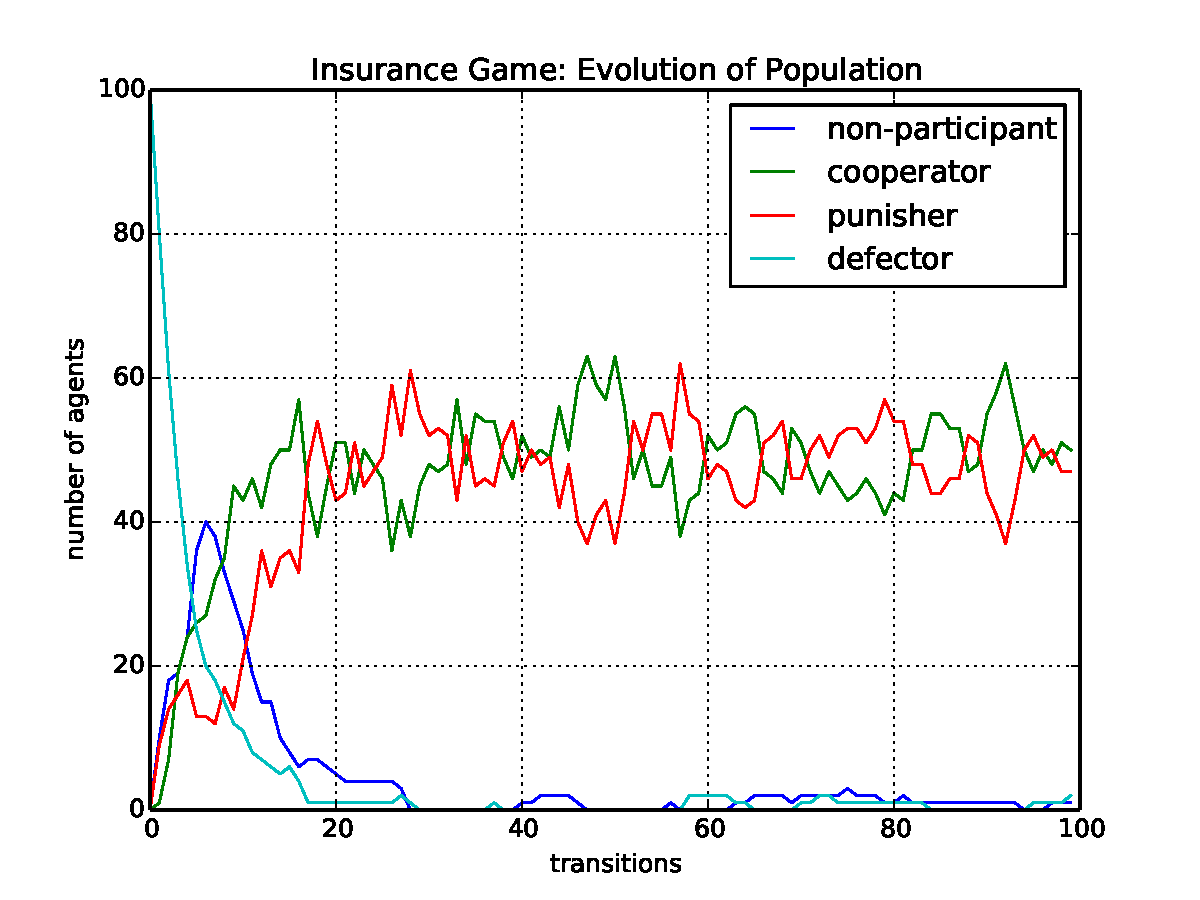
\includegraphics[scale = 0.4]{10.pdf}
 \end{subfigure}
 \begin{subfigure}{.5\textwidth}
   \label{}
   \centering
   \caption{The evolution of rewards: basic insurance game}
   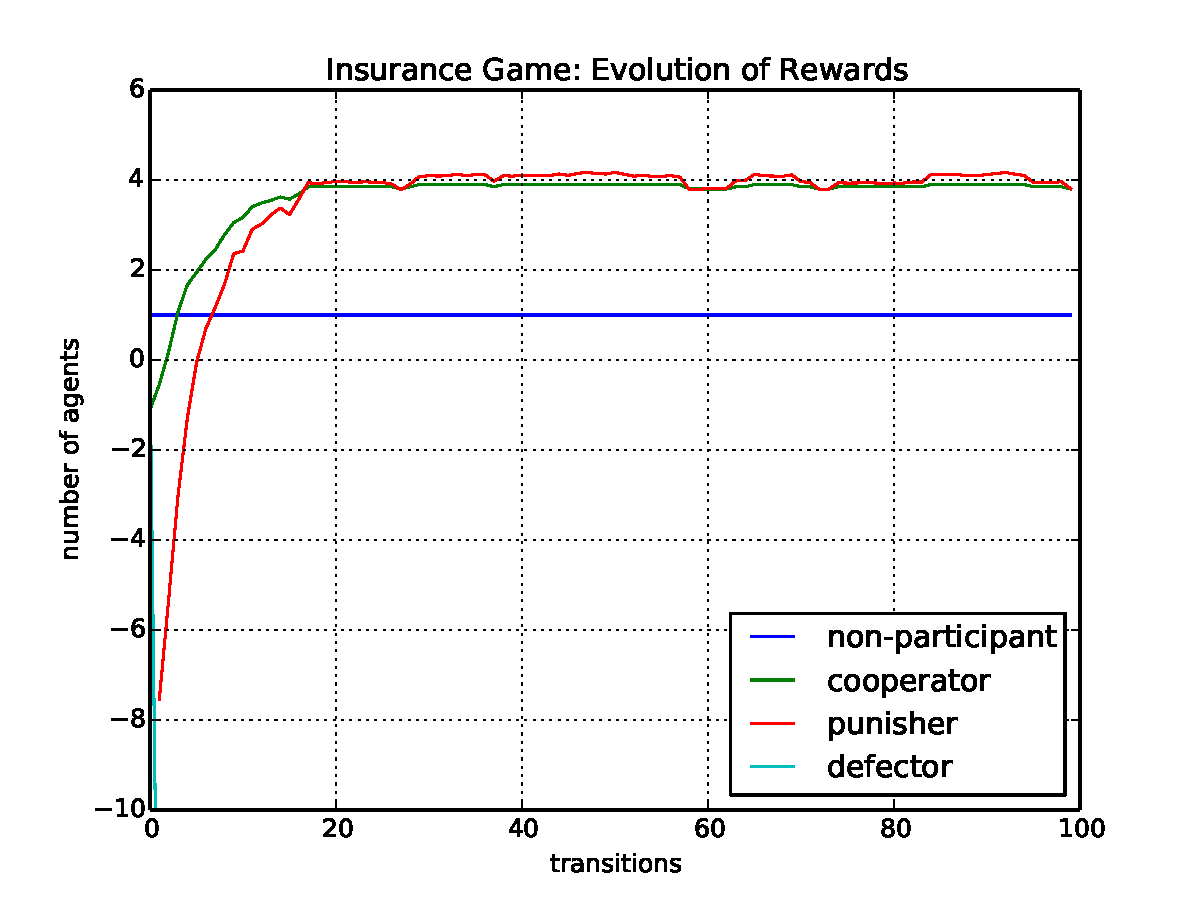
\includegraphics[scale = 0.4]{11.pdf}
 \end{subfigure}
\end{figure}
%%%%%%

As seen in Figure 4, the enforced insurance policy worked as a catalyst for the evolution by keeping the system stable. First of all, it made the transient period shorter by changing it from ~60 transitions to ~20 transitions (Figure 1(a) and Figure 4(a)). As every agent pays a small amount for the good of public punishment, the reward of punishers increased rapidly. Meanwhile, the effect can be seen in the less fluctuating transient stage at the beginning.
\subsection{Effect of geographic constraint and insurance}
%%%%%%%
\begin{figure}[!h]
 \caption{Geographically constrained insurance game}
 \begin{subfigure}{.5\textwidth}
   \centering
   \caption{The evolution of agents: geographically constrained insurance game}
   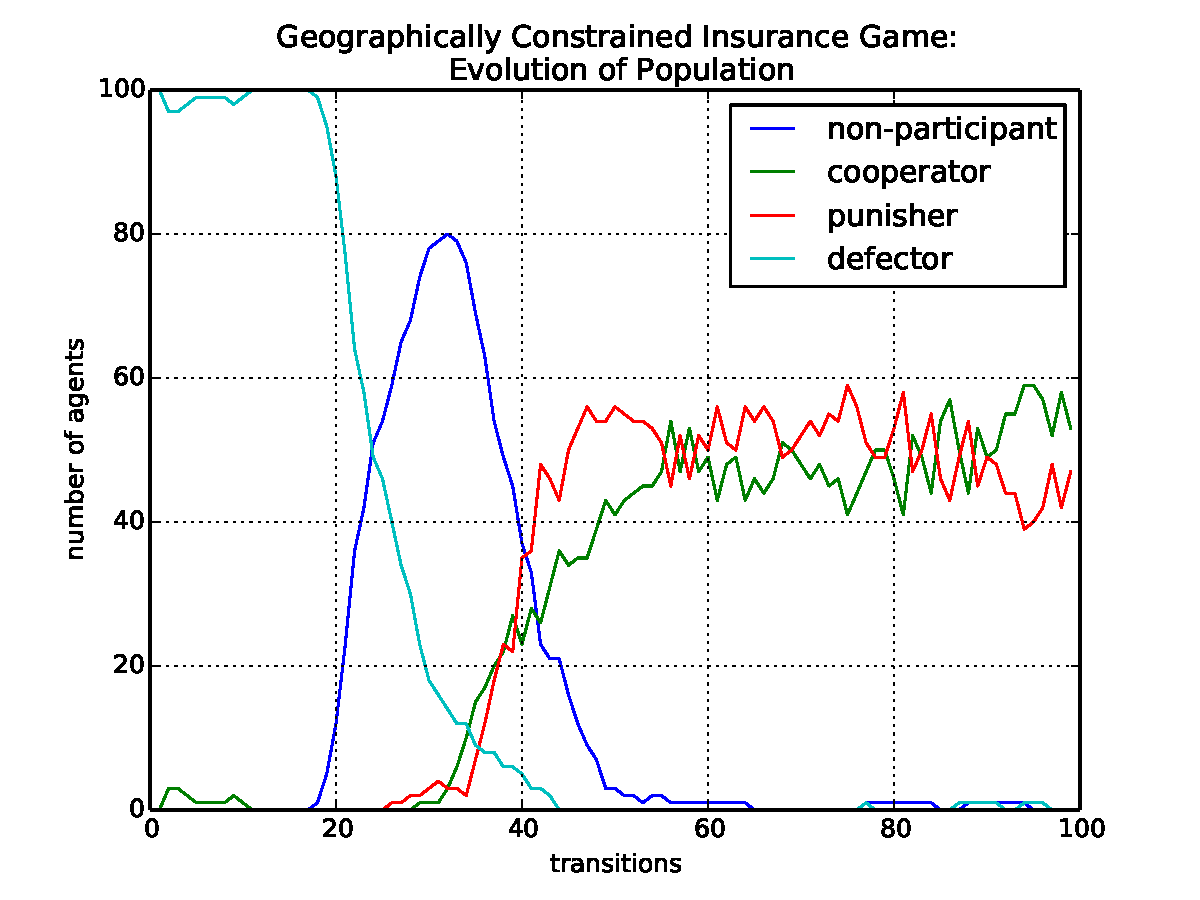
\includegraphics[scale = 0.4]{14.pdf}
 \end{subfigure}
 \begin{subfigure}{.5\textwidth}
   \centering
   \label{}
   \caption{The evolution of rewards: geographically constrained insurance game}
   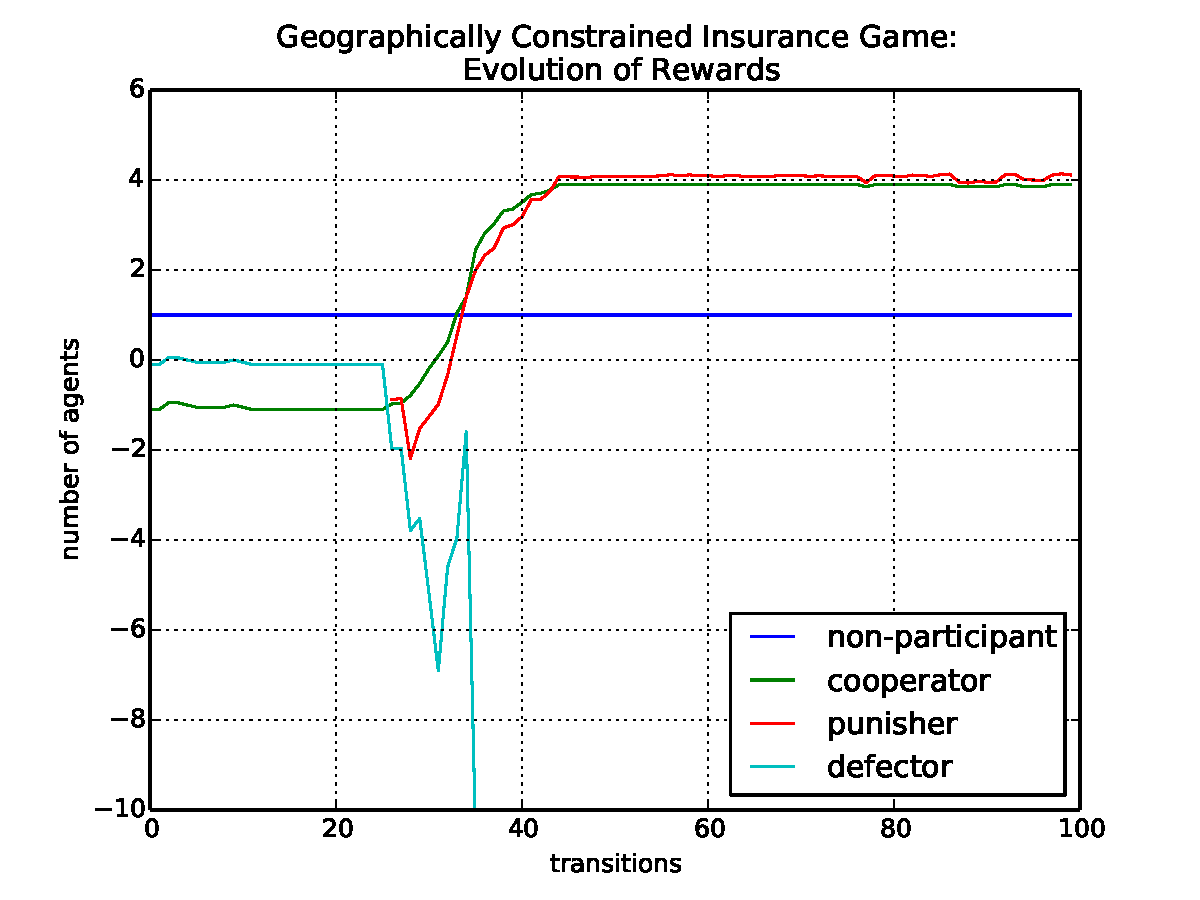
\includegraphics[scale = 0.4]{15.pdf}
 \end{subfigure}
\end{figure}
%%%%%%%%%%check to see if the papragraph make sense.
We have combined geographic constraint and insurance policy in our game model. The impact when both factors work together is largely depend on the parameters, i.e. the radius of geographic constraint and the amount of insurance. These two factors are counteractive, hence the game became more unpredictable. Figure 5 shows one instance of geographically constrained insurance game. Interestingly, there was a plateau period from the start to the 20th iteration in the game initialized by 100 defectors. This phenomenon was caused by the incomplete information. Every agent remained to be defector as there were no more agent seen who better performed. The population started to shift as there were non-participants emerged due to the mutation rate. From the start to 15th transition, there was a small wave of cooperators. These group of cooperators did not survive since cooperators must depend on punishers to increase their rewards. Insurance policy plays a role in this game such that the punishers evolve faster than in basic geographically constrained games (Figure 2(a) and Figure 5(a)).


\section{Discussion}

\subsection{Different initialization condition}
Figure 6 compares two instances of basic geographically constrained insurance game with four different initializations. The punishers always thrived regardless of the initial stages. The only situation where punisher might not be a good choice is when the cooperation is taken over by defectors and non-participation is obviously an alternative. This makes sense since, if a cooperation is so hopeless, it's unreasonable to stay. Unlike basic game, punishers are much stronger and easy to survive in this case.

\subsection{How close are models to realities?}
The human society is a very complicated system, with far more variables and interactions than can be modeled. It is interesting when we try to recover society behaviors with simple models. Can we really gain any insight or prove anything about reality with these simple models? It would also be interesting to see if we can collect real data, fit the parameters in these simple models. But the question remains, how much we can trust the prediction by these models. Another question to ask is, is there really such an abstraction of one aspect of the society, i.e., can we find a projection onto some low dimensional space of the human society, such that the projection is simple and predictable by a model. The project stimulated us to think a lot about the effectiveness of modeling.

\subsection{Sensitivity to parameters}
The behavior of insurance games are less sensitive than basic games. However, the parameters have to be within a certain range such that the criterions at the end of Section \ref{sec:game_type} is met. If case of one criterion is broken, such as the 2) one, non-participants will take over and it will be a whole different senario. People might ask that, why is the human society falls into the right region, where punishers and cooperation is the final steady-state? The answer is, we don't. In the history, there emerged many cooperations and punishers whose parameters did not fall in this right region, and they vanished. 

\begin{figure}[!h]
 \caption{Comparison of the initialization}
 \begin{subfigure}{.5\textwidth}
   \centering
   \caption{The evolution of agents: basic geographically constrained game (initialized by 100 defectors)}
   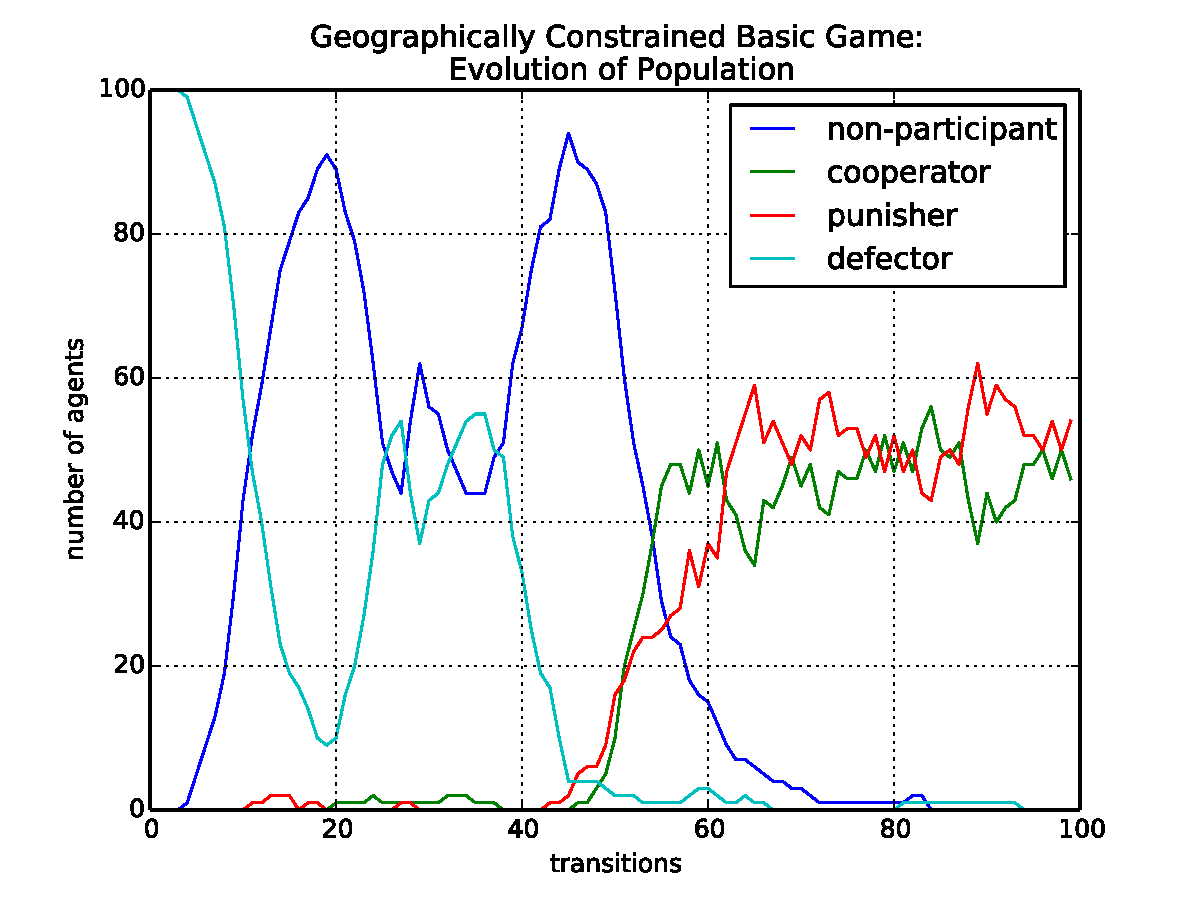
\includegraphics[scale = 0.4]{4.pdf}
 \end{subfigure}
  \begin{subfigure}{.5\textwidth}
   \label{}
   \centering
   \caption{The evolution of rewards: basic geographically constrained game (initialized by 100 cooperators)}
   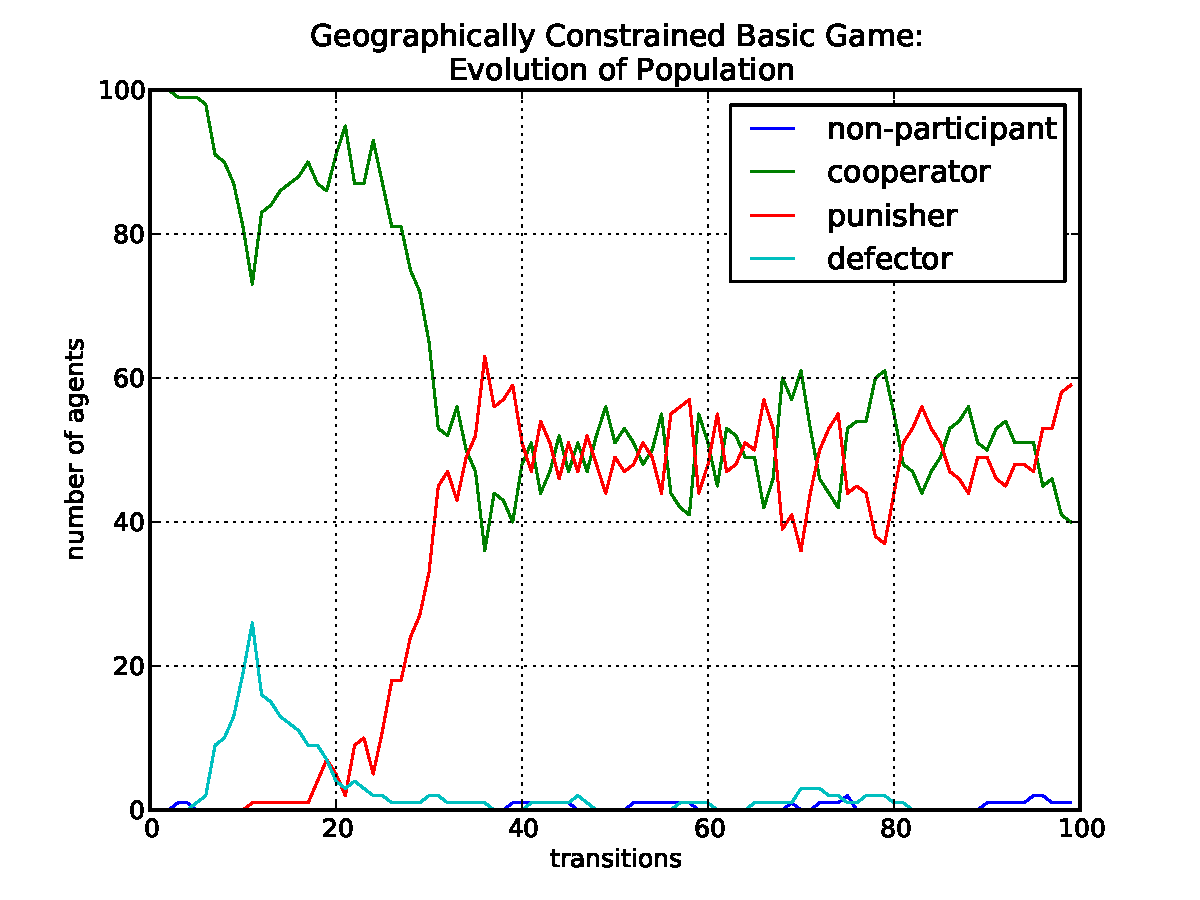
\includegraphics[scale = 0.4]{12.pdf}
 \end{subfigure}
 \begin{subfigure}{.5\textwidth}
   \label{}
   \centering
   \caption{The evolution of rewards: basic geographically constrained game (initialized by 99 cooperators and 1 defector)}
   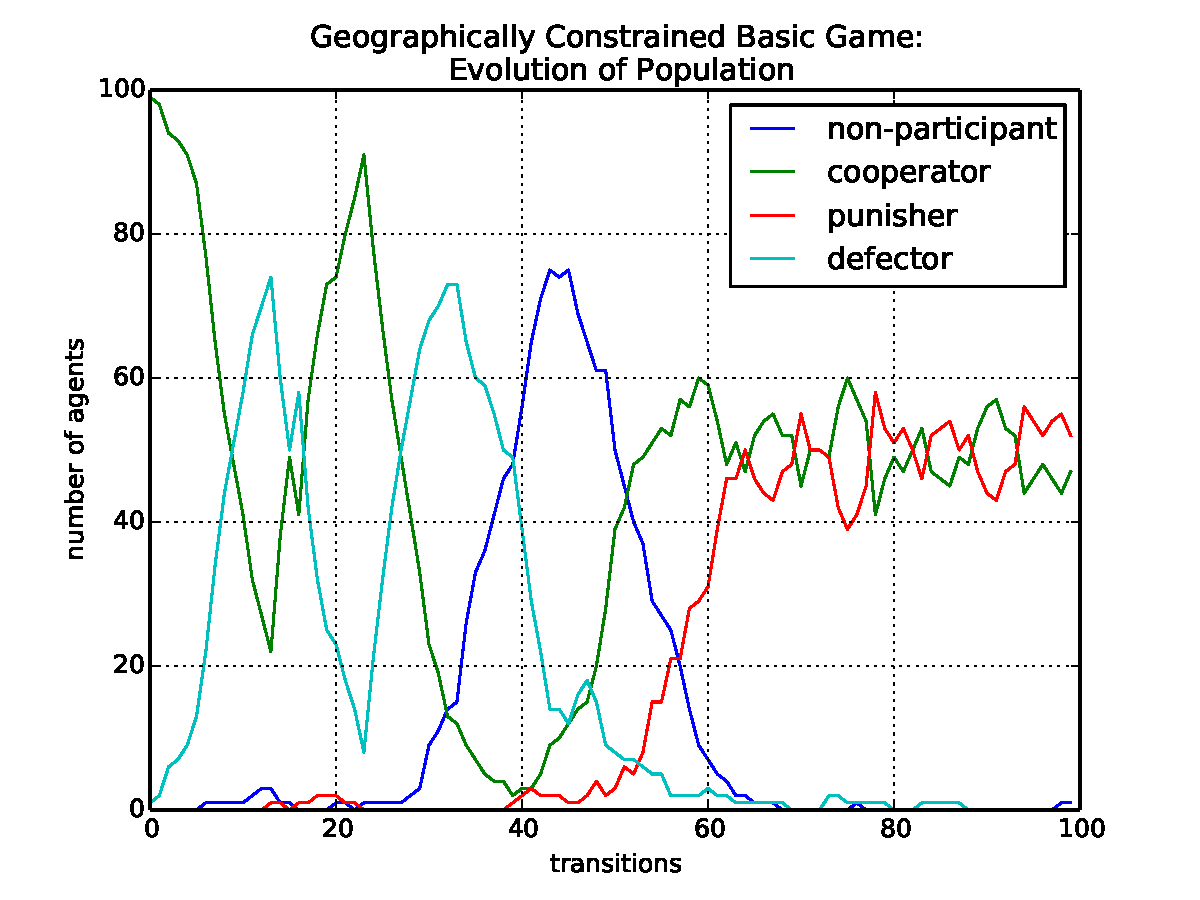
\includegraphics[scale = 0.4]{6.pdf}
 \end{subfigure}
 \begin{subfigure}{.5\textwidth}
   \centering
   \label{}
   \caption{The evolution of rewards: basic geographically constrained game (initialized by 100 non-participants)}
   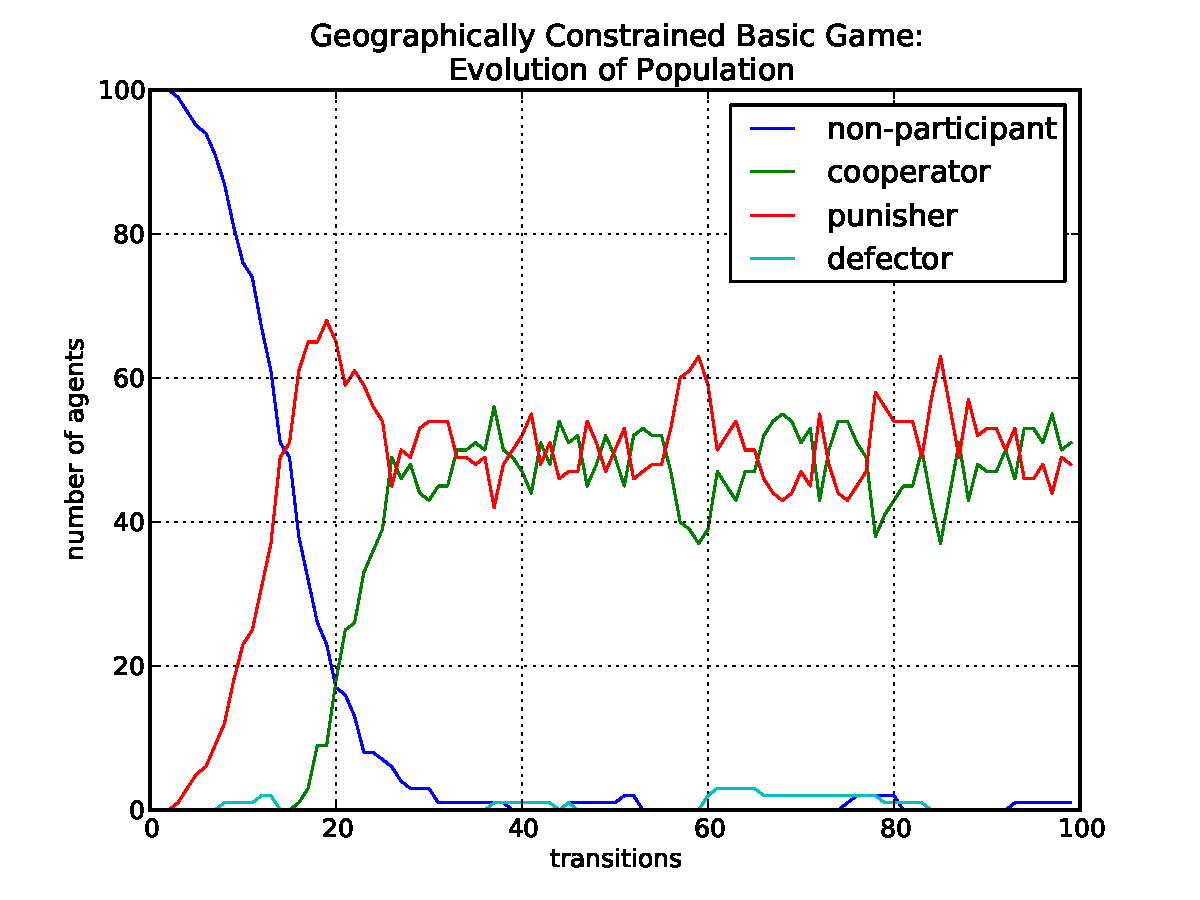
\includegraphics[scale = 0.4]{13.pdf}
 \end{subfigure}
\end{figure}

\section{Conclusion and Future Works}
The previous study has demonstrated the mechanism of the thriving of punishers, and pointed out the importance of voluntary participation. We were inspired by this model and would like to incorporate more features in order to explain the two real-world examples: the restricted communication and the enforced tax (or insurance) policy. We have successfully established a model in python and added these new variations. To sum up, our model reiterated the evolutionary advantage of voluntary punishers. We also proved the inhibiting effect of geographic constrain and the catalyzing effect of insurance policy. The model could be utilized in organizational and developmental research such as the optimization of tax policy and the communication strategy in underdeveloped rural area.

Likewise, our model was based on a series of assumptions. Our model bears the same assumptions with the previous study including excludable cooperative goods, constant pay-off of the non-participants, and ignorance of the economics of the scale. Additionally we have not considered the mobility of the agents, the preservability of public goods, as well as the competition of multiple enterprises. These limitations will be addressed in future works.

\subsection{Multiple cooperations}
Further on we can split agents according to location or connection constraints into different cooperations, where agents can choose to join different cooperations or stay as non-participant. Cooperations reward can also differ due to their sizes. Incorporating these features, we believe we can simulate interactions between companies, such as large companies gradually expand, turning everyone into its member and distroying smaller companies. We are also expecting cooperations with punishers are more desirable.

\subsection{Accommodation and mobility of agents}
In real world, people are always traveling or relocating, changing the dynamics of local world. If we allocate natural resources growth over the whole region, make agents reward also depending on the resource and allow agents to travel, then it would be another interesting simulation.

\bibliographystyle{ieeetr}
\bibliography{ref}

\end{document}
